\pagestyle{fancy}
\fancyhead{}
\fancyhead[L]{Chapter \thechapter}
\fancyhead[RO,RE]{Distributed Task-based In Situ Data Analytics for High-Performance Simulations}
\fancyfoot{}
\fancyfoot[RO,LE]{\thepage}



\chapter{Introduction}\label{chap:intro}
\vspace{20mm}
\epigraph{\textit{ What would life be if we had no courage to attempt anything?}} {Viencent Van Gogh}

\newpage

\section{Introduction}

\begin{wrapfigure}{l}{0.35\textwidth}
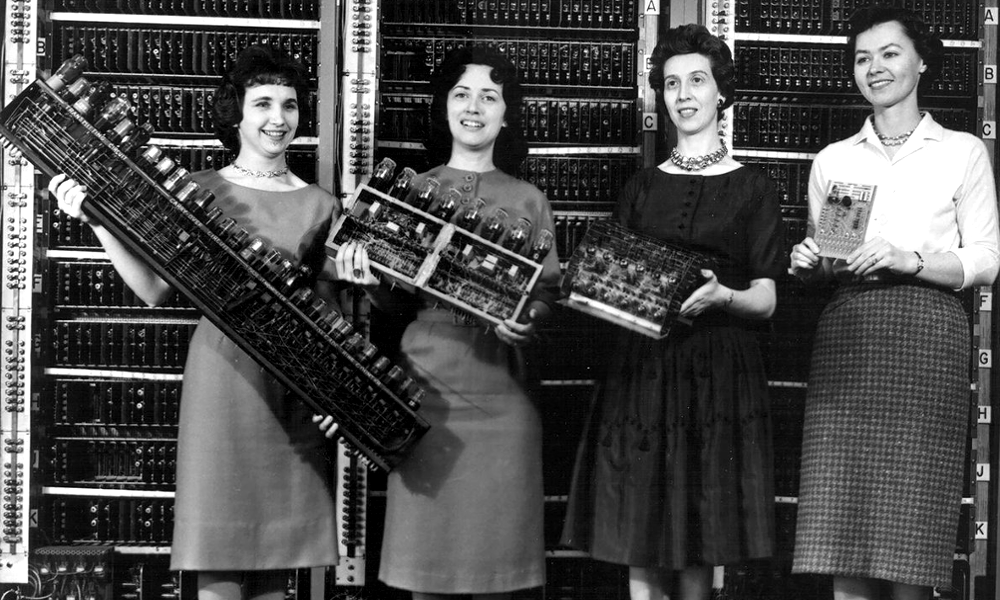
\includegraphics[width=0.9\linewidth]{figures/ENIAC-team.png}
\caption{ENIAC team, (Figure from~\cite{eniac}).}
\label{figeniac}
\end{wrapfigure}


The term of \textit{supercomputers} was used for the first time in March 1920, in the New York World, to refer to \textit{"new statistical machines with the mental power of 100 mathematicians in solving even highly complex algebraic problems"}~\cite{schneck_supercomputer_1987}. Since then and over the last 70 years, computing has grown from the first programmable electronic general-purpose computer: the Electronic Numerical Integrator and Computer (ENIAC, Figure~\ref{figeniac}~\cite{eniac}) able to process 500 floating-point operations per second (flops), completed in 1945 to the first Exascale supercomputer in the world: Frontier (Figure~\ref{figfrontier}~\cite{frontier-image}) able to process 1.102 Exaflops~\cite{top500, frontier}. 

One can ask for a simple definition of high-performance computing and question the need for supercomputers while a laptop is enough for our daily tasks. There are several answers to the first question, and here we have chosen the two that seem to be the most relevant to us.   
A high-performance computer is defined in the JISC New Technology Initiative Proposal~\cite{JISC} and cited in~\cite{hpc} as:
\textit{"computing resources which provide more than an order of magnitude more computing power that is normally available on one's desktop"} 
And high-performance computing is defined on the IBM website~\cite{ibm}: 
\textit{"HPC is technology that uses clusters of powerful processors, working in parallel, to process massive multi-dimensional datasets (big data) and solve complex problems at extremely high speeds. HPC systems typically perform at speeds more than one million times faster than the fastest commodity desktop, laptop or server systems."}
The two definitions are complementary, and both of them mention the computing power and the memory size of supercomputers, which leads us to answer the second question regarding the need for supercomputing. It arises to solve complex, memory/compute-bound problems. 

%However, before we go further, we would like to quote another citation from the "National High-Performance Computer Technology Act" (a.k.a the "Gore Bill")~\cite{nitecki_influence_2008}: 
%\textit{"The nation which most completely assimilates high-performance computing into its economy will very likely emerge as the dominant intellectual, economic, and technological force in the next century"}. 


Today, supercomputing is involved in the research for solutions to an extensive list of challenges: green and renewable energy, nuclear fusion, solar and water energy, and medical concerns ranging from understanding the human body to drug discovery thanks to computing power that speeds up the research process. Examples from astrophysics, trying to understand our universe, chemistry and the creation of new materials, simulating natural phenomena or coupling real experiments and the Internet of Things (IoT) with HPC to form digital twins systems.
Several legacy problems started to be resolved with the emergence of HPC, thanks to the computing power and memory they offer. For instance, the use of machine learning and artificial intelligence has gained in popularity since the appearance of the general-Purpose graphic processing unit (GPGPU). Similarly, alongside telescopes, HPC has been used to understand and explore the theoretical aspects of a black hole, and in 2019 the first-ever black hole image could be synthesized~\cite{erotokritou_hpc_2019}.     

\begin{wrapfigure}{br}{0.35\textwidth}
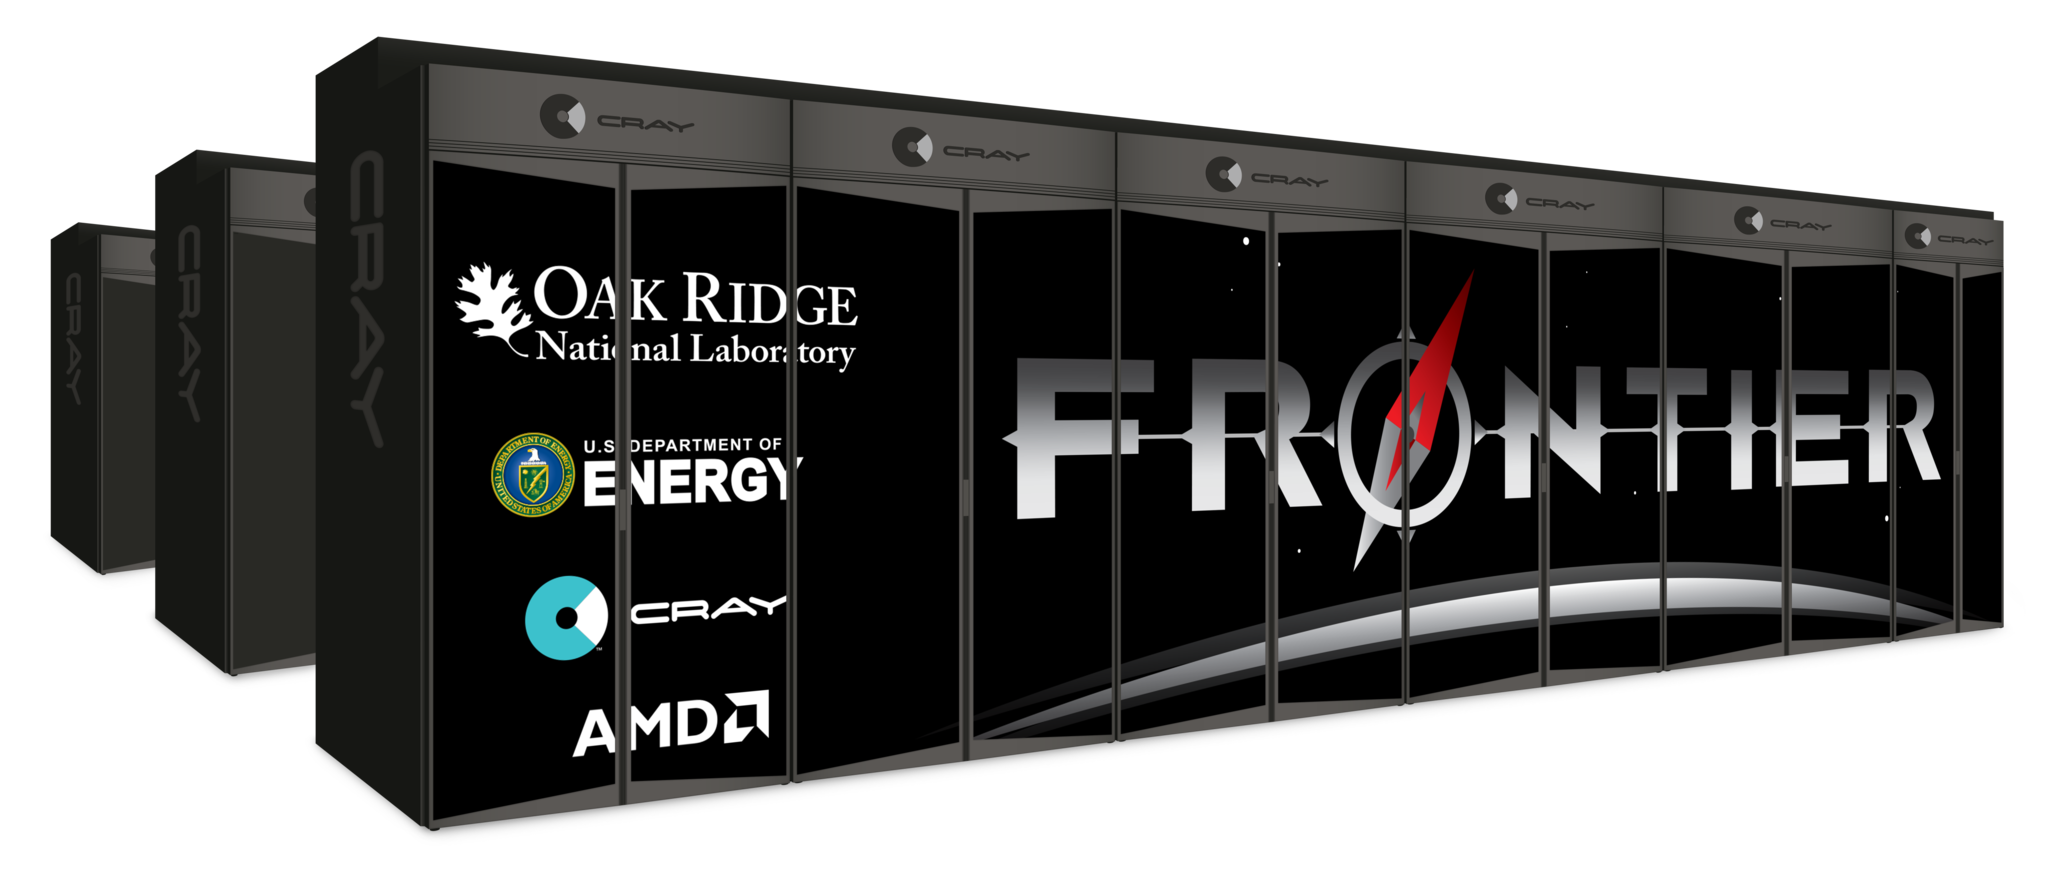
\includegraphics[width=0.9\linewidth]{figures/Frontier.original.png}
\caption{Frontier the first Exascale supercomupter, (Figure from~\cite{frontier-image})}
\label{figfrontier}
\end{wrapfigure}

According to J. Dongarra~\cite{dongarra_trends_2006}, the value of a supercomputer derives from the value of the problem it solves. As such, supercomputing is tightly related to scientific applications that are usually simulations. Those programs that model physics phenomena are complex and need large amounts of both computing power and memory to run. 
To achieve such a performance, computer architecture has evolved from a simple implementation of a Von Neumann computer to millions of powerful cores and accelerators interconnected together, able to process hundreds of petaflops per second. Along with those complex architectures, different programming models are proposed to write efficient programs.   

High-performance simulations are typically iterative programs that evolve over time and may produce, in some fields, such as weather forecasts, dozens of terabytes per hour.   
The generated data needs to be processed to understand the phenomenon under study. 
In the classical workflow, the data generated by the simulation is first written to disk and then read back for post-processing, also known as post hoc processing, usually on a different workstation. 
Data analytics are easily performed with sequential Python codes, recently scientists adopted available parallel libraries adapted for data and big data analytics because of the huge amount of data generated by simulations. 

The size of the output is not the only challenge. While CPU performance has increased following Moore's law, disk bandwidth did not, and the gap between them is widening by a few orders of magnitude, creating what is known as the IO bottleneck. 
In situ workflows were introduced in 2008. They aim to process the data generated by large-scale simulations as close as possible to when (time) and where (memory) it was generated. Such workflows bypass disk accesses by processing the data in the same supercomputer as the simulation, thus avoiding the previously mentioned IO bottleneck. 
Despite the performance shown by in situ workflows, they are not widely used in the community because of their setup complexity and the need for prior knowledge about data analytics to do.  

Most of the existing in situ tools are built on the MPI programming model inherited from the host simulation. While this model, alongside others known as MPI+X, is well suited for scientific applications for their regularity, they are not adapted for data analytics purposes. 
Data analytics algorithms have a different structure compared to simulations. They are characterized by irregular data and control structures and communication patterns. Trying to write some of those algorithms in a static and synchronous model such as MPI is like putting the square peg in a round hole. Not only are they not compatible, but also, putting them together is complex.

In this work, we want to bring together post hoc simplicity and in situ performance. In other words, we will couple high-performance simulations parallelized in MPI with in situ analytics written in a more adapted model of data analytics algorithms, namely distributed task-based programming model. 

The rest of the document is organized as follows.
\begin{itemize}

    \item \textbf{Part I State of the Art.} It contains two chapters. In Chapter 2, we present the context and related work, namely in situ and distributed task-based frameworks. In Chapter 3, we present the tools used in this work, namely \pdi and \dask distributed.    

    \item \textbf{Part II Contributions.} It presents the main scientific contributions of this work and contains five chapters. Chapter 4 presents the approach that we propose, called \deisa bridging model with the first elements of its implementation using \dask and \pdi. Chapter 5 presents a complete implementation, with the needed configuration and user API. Chapter 6 proposes conceptual improvements in \deisa and \dask distributed. 

    \item \textbf{Part III Conclusion and Perspectives.} It summarizes the main conclusions and lessons learned from this work, and provides feedback about possible perspectives and projects. 
    
\end{itemize}
    
%\newpage

% \section{Objectives}
% First of all, this work has been motivated by a necessity that gave rise to a need: a necessity to switch to in situ workflows to bypass disk accesses and thus the IO bottleneck, then the need for easiness and productivity in writing in situ workflows. Our goal is to bring together post hoc easiness and in situ performance. In other words, our goal is to provide a user-friendly in situ tool that is as easy and with an almost similar interface as post hoc tools.  


%\section{Contributions}

\section{Communications}
\begin{itemize}
  
  \item \textbf{COMPAS21: Conférence francophone d'informatique en Parallélisme, Architecture et Système 2021}

Amal Gueroudji, Julien Bigot, Bruno Raffin. Preliminary Experiments in Coupling in situ \dask analytics with MPI Simulations. COMPAS 2021 - Conférence francophone d'informatique en Parallélisme, Architecture et Système, 2021, virtual

  \item  \textbf{HiPC21:  28th International Conference on High-Performance Computing, Data, and Analytics 2021}

Amal Gueroudji, Julien Bigot, Bruno Raffin. DEISA: \dask-enabled in situ analytics. HiPC 2021 - 28th
International Conference on High-Performance Computing, Data, and Analytics, Dec 2021, virtual,
India. 

  \item \textbf{HPC/DA21:  Workshop on the In Situ Co-Execution of High-Performance Computing \& Data Analysis 2021}

Amal Gueroudji, Julien Bigot, Bruno Raffin. Preliminary Experiments in Coupling in situ Dask analytics with MPI Simulations. HPC/DA 2021 - Workshop on the In Situ Co-Execution of
High-Performance Computing \& Data Analysis, July, 2021

  \item  \textbf{Per3S 2022: 6th Workshop Performance and Scalability of Storage Systems 2022}

Amal Gueroudji, Julien Bigot, Bruno Raffin. Handling IO data with PDI and Optimizing away IO with \pdi/\deisa. Per3S 2022 - 6th Workshop Performance and Scalability of Storage Systems, June 2022


  \item \textbf{PASC22: Conference on The Platform for Advanced Scientific Computing 2022}

Virginie Grandgirard, Kevin Obrejan, Dorian Midou, Y Asahi, PE Bernard, J Bigot, E Bourne, J Dechard, G Dif-Pradalier, P Donnel, X Garbet, A Gueroudji, G Hager, H Murai, Yacine Ould-Ruis, T Padioleau, L Nguyen, M Peybernes, Y Sarazin, M Sato, M Tsuji, P Vezolle. New advances to prepare GYSELA-X code for Exascale global gyrokinetic plasma turbulence simulations: porting on GPU and ARM architectures. PASC22 - Conference on The Platform for Advanced Scientific Computing, the Association for Computing Machinery (ACM); the Swiss National Supercomputing Centre (CSCS), Jun 2022, Bâle (virtual event), Switzerland. pp.1-21. 

  \item \textbf{PDSW22 Work In Progress: 7th International Parallel Data Systems Workshop 2022}
  
Amal Gueroudji, Julien Bigot, Bruno Raffin. \dask-Enabled External Tasks For In Transit Analytics. PDSW 2022 - 7th International Parallel Data Systems Workshop, Nov 2022 

  \item \textbf{JLESC15 Short Talk: 15th Joint Laboratory for Extreme-Scale Computing Workshop 2023}
  
Amal Gueroudji, Julien Bigot, Bruno Raffin. \dask-Enabled External Tasks For In Transit Analytics. JLESC15 2023 - 15th Joint Laboratory for Extreme-Scale Computing Workshop, Mar 2023 

\end{itemize}


\hide{
\subsection{Software\footnote{https://github.com/GueroudjiAmal/deisa}}

\subsubsection{\deisa: \dask-Enabled In Situ Analytics python interface}
\deisa python interface is a python library that implements the code coupler classes to \dask distributed framework. It implements the \deisa bridges and the Adaptor and offers a simple API to use \dask distributed for in situ analytics. It also implements a distributed data structure called \deisa virtual arrays on top of \dask arrays, and contracts to optimize data communications. 

\subsubsection{\pdi \deisa Plugin}
\pdi \deisa plugin is a \pdi plugin implemented in C++ that supports python and uses the \deisa python interface to perform the coupling with \dask distributed. We have provided a declarative way to configure the in situ processing in the same specification tree as \pdi.

\paragraph*{Synchronous Pycall-based \deisa:}
We have provided \deisa functionalities based on the built-in plugin Pycall in \pdi. This version allows a synchronous execution of the in situ analytics. Since the \deisa library is written in python, it is easily used in Pycall. 

\paragraph*{Asynchronous \deisa plugin:}
We have implemented a separate \deisa plugin to perform exclusively in situ analytics with \dask distributed. The plugin is written in C++ and inherits from the \pdi plugin class. It can be loaded and used with other plugins. 

\subsubsection{\dask-Enabled External tasks}
We have provided support for external tasks in \dask distributed in a separate git fork to make \dask naively support the integration of external tasks in its task graph without running into errors. An external task is run outside of \dask cluster, and in our case, it corresponds to simulation tasks.   

}
